\documentclass[a4paper,9pt,twoside]{report}

\usepackage[margin=1cm]{geometry}
\usepackage{amsmath}
\usepackage{titling}
\usepackage{fontspec}
\usepackage{listings}
\usepackage{hyperref}
\usepackage{graphicx}
\usepackage{float}

\usepackage[dutch]{babel}

\usepackage{fontspec}
\setmainfont{Montserrat}

\usepackage{titlesec}

\titleformat{\chapter}[display]{\normalfont\bfseries}{}{0pt}{\Huge}

\title{Nieuwsartikel}

\author{Dylan {Cluyse}}

\begin{document}
	
\chapter{Tech voor taal: Wetenschappelijke artikelen begrijpend lezen met \textit{Pentimentor}.}

\noindent\textbf{Wetenschappelijke artikelen begrijpend lezen is bewezen leesmateriaal in het middelbaar onderwijs. Hoewel deze artikelen scholieren een aanzet tot wetenschappelijk onderzoek kunnen geven, kan het begrijpend lezen van deze materie voor scholieren moeizaam verlopen, vooral scholieren met taalstoornissen. Personaliseerbare tekstvereenvoudiging kan een oplossing bieden. Hoewel het brede publiek niet over een eenduidige oplossing beschikt, kan het prototype \textit{Pentimentor} dit realiseren met de nieuwste taaltechnologieën.}

\medspace

\noindent Plaats jezelf in de schoenen van een scholier in de derde graad van het middelbaar onderwijs. Voor een opdracht begrijpend lezen moet jij het volgende deel uit een wetenschappelijk artikel lezen, afgebeeld op onderstaande simulatie.

\begin{figure}[H]
	\fbox{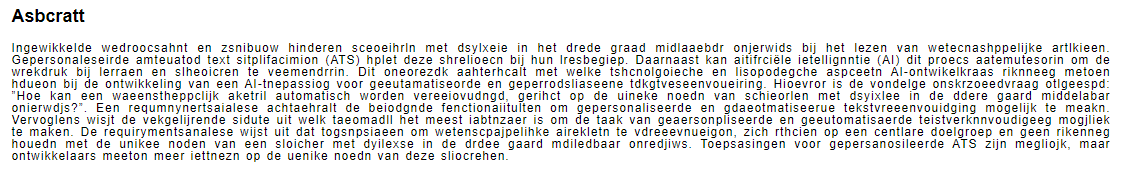
\includegraphics[width=\linewidth]{screenshot-abstract.png}}	
\end{figure}

\noindent Moeilijker dan je denkt? Hoewel symptomen van dyslexie verder gaan dan \textit{dansende letters}, toch benadrukt deze simulatie de stoorzenders waarmee scholieren met dyslexie kunnen kampen. Daarnaast zijn deze artikelen geschreven voor een specifiek vakdomein. Leerkrachten kunnen dit echter aanpakken door de oorspronkelijke tekst te vereenvoudigen. De tekstinhoud blijft echter onaangepast, maar hiervoor kunnen leerkrachten op maat van de scholier vereenvoudigen. In de afbeelding hieronder herschrijf ik de samenvatting door vier technieken toe te passen. 

\begin{enumerate}
	\item De oorspronkelijke weergave aangenamer maken. 
	\item Ongekende of moeilijke woordenschat vervangen naar eenvoudiger synoniemen; als dit niet mogelijk is, voeg het woord samen met de betekenis toe aan een woordenlijst.
	\item Moeilijke zinsyntax herschrijven naar kortere zinnen; zonder de oorspronkelijke betekenis te verliezen.
	\item Tot slot herschrijf ik de oorspronkelijke paragraaf in een ander formaat, in dit geval een opsomming. De inhoud in een tabelvorm schrijven is een andere manier om veel informatie bondig weer te geven.
\end{enumerate}

\begin{figure}[H]
	\fbox{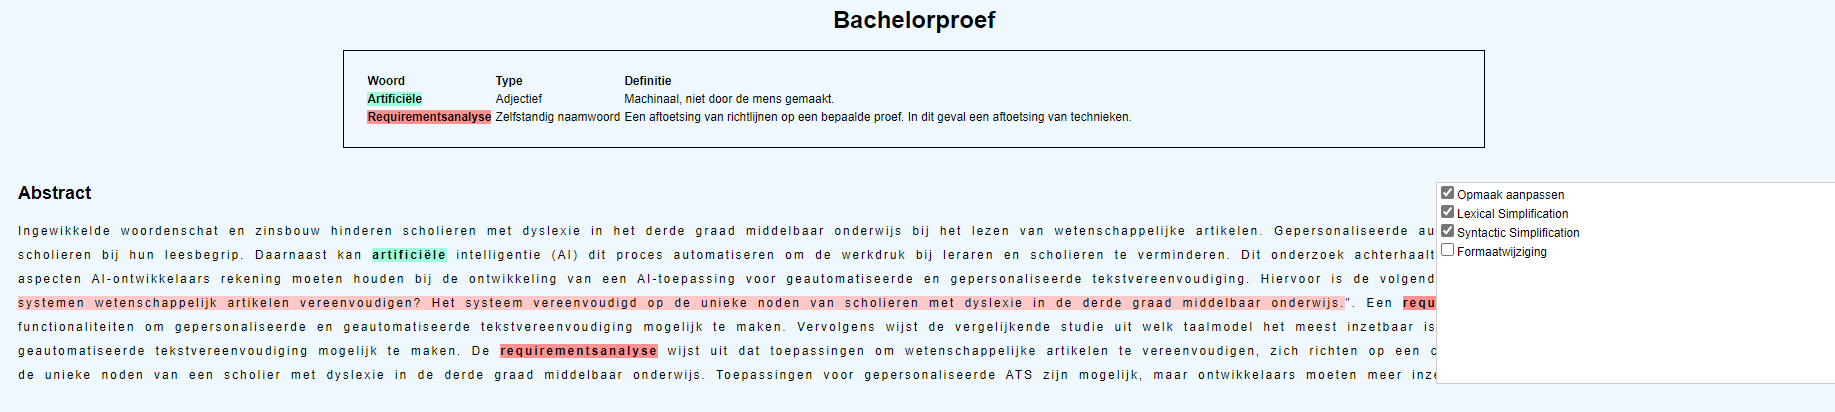
\includegraphics[width=\linewidth]{screenshot-abstract-post.png}}
\end{figure}

\noindent Meer informatie rond de verschillende soorten tekstvereenvoudiging kan u op deze link terugvinden. Echter neemt dit personaliseerbaar proces tijd en energie van de auteur. De vraag blijft: hoe kunnen scholieren en leerkrachten dit proces (bestaande uit de vier handelingen in de bovenstaande afbeelding) automatiseren; en kunnen ontwikkelaars hier een inbreng in maken?

\subsubsection{Welke tools kan jij gebruiken om teksten automatisch te laten vereenvoudigen?}

\noindent Allereerst neemt de overheid initiatief om scholieren met taalstoornissen te ondersteunen. Zo lenen zij toepassingen uit die vooral het lezen van wetenschappelijke artikelen kan bevorderen, zoals Alinea en Kurzweil. Dit doen ze door de tekst in een personaliseerbaar formaat te gieten wat scholieren met dyslexie baat. Toch kunnen deze toepassingen géén tekstinhoud vereenvoudigen.

\medspace

\noindent Handmatig wetenschappelijke artikelen herschrijven is een taak op zich. Hoewel dit proces door een machine laten doen op maat van een ontelbaar aantal studenten een moeilijke taak is, toch kunnen een handvol toepassingen dit mogelijk maken. SciSpace en Simplish kan iedereen online beschikken. Deze toepassingen kunnen de tekstinhoud aanpassen, maar kunnen de weergave van de tekst niet aanpassen op maat van de scholier.

\medspace

\noindent Opkomende chatbots zoals Bing Chat en ChatGPT tonen ook hun mogelijkheden door tekst te herschrijven op het niveau van de mens. De achterliggende systemen tonen potentieel én zijn beschikbaar voor ontwikkelaars. Toch moeten gebruikers niet-intuïtieve stappen afleggen; daardoor zijn deze toepassingen niet eenduidig genoeg voor het grote publiek. Onderzoek naar dergelijk toepassingen is van essentieel belang en kan revolutionair zijn, want deze doelgroep heeft hier duidelijk nood aan. Daarnaast kunnen scholieren zonder taalstoornissen baten van dergelijk toepassingen, want dit helpt hen bij het begrijpend lezen van moeilijke materie.

\subsubsection{Hoe kunnen ontwikkelaars teksten vereenvoudigen?}

\noindent Als huidige toepassingen er niet in slagen om een eenduidige toepassing te ontwikkelen, hoe kunnen ontwikkelaars dit dan wél doen? Hiervoor komen taalmodellen aan de pas. Vrij beschikbare taalmodellen kunnen de moeilijkheidsgraad van de tekst verlagen, maar kunnen de tekstinhoud niet interpreteren of omvormen naar een ander formaat. 

\medspace

\noindent GPT-3, of het achterliggende taalmodel van Bing Chat en ChatGPT, doet dit wél en vormt daarmee een revolutionaire bouwsteen voor automatische tekstvereenvoudiging. Echter zijn deze toepassingen voor de gewone scholier of leerkracht nog te ingewikkeld om te gebruiken. Hoewel het taalmodel potentieel toont, toch moeten ontwikkelaars een omgeving maken die deze technologie toegankelijk maakt voor het grote publiek. Dat doet \textit{Pentimentor}.

\subsubsection{Wetenschappelijke artikelen begrijpend lezen met \textit{Pentimentor}}

\noindent \textit{Pentimentor} toont aan dat ontwikkelaars met eenduidige tools dergelijk systemen kunnen ontwikkelen voor het onderwijs. Met gratis tools kan het systeem de tekst uit een ingediend wetenschappelijk artikel ophalen, alsook kan het systeem de tekst naar een nieuw formaat schrijven, zowel als word-document en pdf-document. Systemen hebben bijvoorbeeld moeite bij het inlezen van oude wetenschappelijke artikelen. Daarom maakt het systeem gebruik van een geavanceerde methode die wél de tekst kan ophalen.

\medspace



\medspace

\noindent Ook jij kan dit prototype uitproberen. Op deze link kan u een stappenplan volgen om van deze toepassing gebruik te kunnen maken. Tenslotte doe ik een warme oproep aan (toekomstige) onderzoekers in het logopedisch of onderwijsvakgebied. Zo kunnen onderzoekers met dit prototype de effecten bij het begrijpend lezen van dergelijk artikelen bij verschillende doelgroepen uittesten.

\end{document}